\documentclass[final]{beamer}
\usepackage[size=a3,orientation=landscape, scale=1.1]{beamerposter}
\usepackage{graphicx}
\usepackage{lipsum}
\usepackage[scaled]{helvet} % Helvetica font
\renewcommand\familydefault{\sfdefault} 

\usepackage{amsmath}
\usepackage{graphicx}
\graphicspath{{images/}}
\usepackage{svg}
\svgsetup{inkscapelatex=false} % - does not use the latex fonts in imported svg

\usepackage{lmodern}
\usepackage{array}  % Allows for more flexible column formatting
\usepackage{booktabs}  % Improves table aesthetics
\usepackage[skip=0.5ex, justification=raggedright, singlelinecheck=false]{caption}
\usepackage{enumitem}
\usepackage{float} % Required for the H specifier
\usepackage{subcaption} % Required for sub-figures

% table
\usepackage{multirow}
\usepackage{tabularx}
\usepackage{booktabs}


\PassOptionsToPackage{colorlinks=true, allcolors=blue}{hyperref}
\usepackage[style=apa, backend=biber]{biblatex}

\addbibresource{main.bib}

\newcommand{\getyear}[1]{\citeyear{#1}}

% Setup a minimalistic theme
\setbeamertemplate{navigation symbols}{}
\setbeamercolor{block title}{bg=white,fg=black}
\setbeamercolor{block body}{bg=white,fg=black}

% Metadata
\title{Processing}
\author{Tibor Udvari} 
\institute{HEAD – Genève}
\date{\today}

\setbeamercolor{chcolor}{bg=black,fg=white}
\setbeamertemplate{headline}{
  \begin{beamercolorbox}[wd=\paperwidth, ht=4cm, dp=1ex,center]{chcolor}
    \vbox to\headheight{\vfil
        \vskip0.25cm  % Adjust this value to shift text up or down
      \centering
      \Large Charting the Beginnings of the Processing Community\\Implications for Collaborative Open Source Art Development \\
      Tibor Udvari, HEAD Genève
      \vfil}
  \end{beamercolorbox}
}

\setbeamertemplate{footline}{
  \hspace{3em}  % Padding on the left side
  \begin{beamercolorbox}[wd=\paperwidth, ht=1.5cm, dp=0.5cm]{footcolor}
    \begin{minipage}{.15\paperwidth}  % Reduced to 15% of paper width
      \hspace{1em}  
      Tibor Udvari / tibor.udvari@etu.hesge.ch
    \end{minipage}
    \hfill
    \begin{minipage}{.3\paperwidth}  % Increased to 30% of paper width
      %tibor.udvari@etu.hesge.ch
    \end{minipage}
    \hfill
    \begin{minipage}{.55\paperwidth}  % Reduced to 20% of paper width
      %HEAD Genève

    \end{minipage}
    \hfill
    \begin{minipage}{.20\paperwidth}  % Reduced to 25% of paper width
      \hphantom{...............................................................................................................} \today

    \end{minipage}
    
    \hspace{4em}  % Padding on the right side
  \end{beamercolorbox}
}


\begin{document}
\begin{frame}[t]
  \begin{columns}[t]
    \begin{column}{.32\textwidth}
      \begin{block}{Introduction}
        \vspace{1.25em}
        \begin{quote}
          "The processing project is a community, a piece of software that you run, and a language. And that order is important." – Ben Fry \parencite[19:22]{artsatmit2017CASTSymposium2017}
          \end{quote}
          \vspace{0.75em}

          The Processing project serves as an intriguing case study in open source development within the intersecting domains of art and technology. While its software and programming language enable artists and developers to create visual artworks, it is the community of contributors that fuels its continued growth and innovation. This study aims to explore the motivations and activities of these contributors by employing a blend of quantitative and qualitative research methods. 
          \smallskip  % Adds a small vertical space for a new paragraph

          Using descriptive statistics of Git commits and forum contributions, supplemented by interviews and forum text analysis, I seek to unravel the dynamics that drive collaborative development in this unique open source project. Our findings offer valuable insights for both the fields of open-source development and digital art creation.
      \end{block}
      \begin{block}{Data Sources}
        \begin{table}[h]
    \raggedright
    \caption{Data sources}
    \label{table:data-sources}
    \begin{tabular}{l l l c}
        \toprule
        Name & Type & Status \\
        \midrule
        Processing alpha forum & Forum & Parsed \\
        Processing beta forum & Forum & Parsed  \\
        Processing 1.0 forum & Forum & Downloaded \\
        Processing 2.0 and 3.0 forum & Forum  & Not downloaded \\
        Current processing forum & Forum & Not downloaded\\
        Github project & Commit history & Parsed \\
        Processing Release Data & Release notes & Parsed \\
        Github Release Data & Release notes \& download statistics & Parsed \\
        Processing libraries\textsuperscript{*} & Software release information & Parsed \\

        \bottomrule
        \multicolumn{3}{l}{\footnotesize \textsuperscript{*}Note: The data set was reconstructed from the processing website archive and is not complete.}
    \end{tabular}
  \end{table}        
      \end{block}
      \smallskip  % Adds a small vertical space for the accompanying text
  
      The research draws upon multiple data sources to form a comprehensive picture of the Processing community and its development practices. These range from forum discussions at various phases of the project to commit histories and issue trackers. The parsing status indicates the extent to which each data source has been prepared for analysis. This multi-faceted approach allows us to delve deeply into both the social and technical aspects of the community.
    
    \end{column}
    \begin{column}{.32\textwidth}
      \begin{block}{Git Commits}
        \begin{figure}[h!] 
    \centering 
    \includesvg[pretex=\sffamily\fontsize{5.58pt}{8pt}\selectfont, width=1\textwidth, keepaspectratio]{images/figure-top12-github.svg}
    \caption{Top 12 source code contributors by number of commits}
    \label{fig:top12-github}  
  \end{figure}
        The primary contributor, also one of the co-founders of Processing, has been responsible for the majority of commits to the main code repository to date.
      \end{block}
      \begin{block}{Forum Posts}
        \begin{figure}[h!] 
    \centering 
    \includesvg[pretex=\sffamily\fontsize{5.58pt}{8pt}\selectfont, width=1\textwidth, keepaspectratio]{images/figure-forum-posts.svg}
    \caption{Top 12 authors by number of posts (Aggregated alpha and beta forum)}
    \label{fig:forum-posts}  
  \end{figure}
        Although Ben Fry remains the most active contributor in forum discussions, the activity distribution is more balanced compared to Git commits. This may be due to the broader range of topics discussed, including technical issues and bugs.
      \end{block}
    \end{column}
    
    \begin{column}{.32\textwidth}
      \begin{block}{Libraries}
        \begin{figure}[h!] 
    \centering 
    \includesvg[pretex=\sffamily\fontsize{5.58pt}{8pt}\selectfont, width=1\textwidth, keepaspectratio]{images/figure-libraries.svg}
    \caption{Distribution of Libraries in the Processing Project}
    \label{figure:libraries}  
  \end{figure}
        %The figure maps out the extensive range of 150 libraries in the Processing project, distributed across 18 distinct categories. Each point on the graph marks a different released version, while the colors signify individual libraries. This visual representation underscores not only the scope and diversity but also the evolutionary history of libraries developed by the community.

      \end{block}
      \begin{block}{Forum vs Git Activity}
        \begin{figure}[!htbp] 
    \centering 
    %\includesvg[pretex=\sffamily\fontsize{5.58pt}{8pt}\selectfont, width=1\textwidth, keepaspectratio]{images/figure-forum-git-activity.png}
    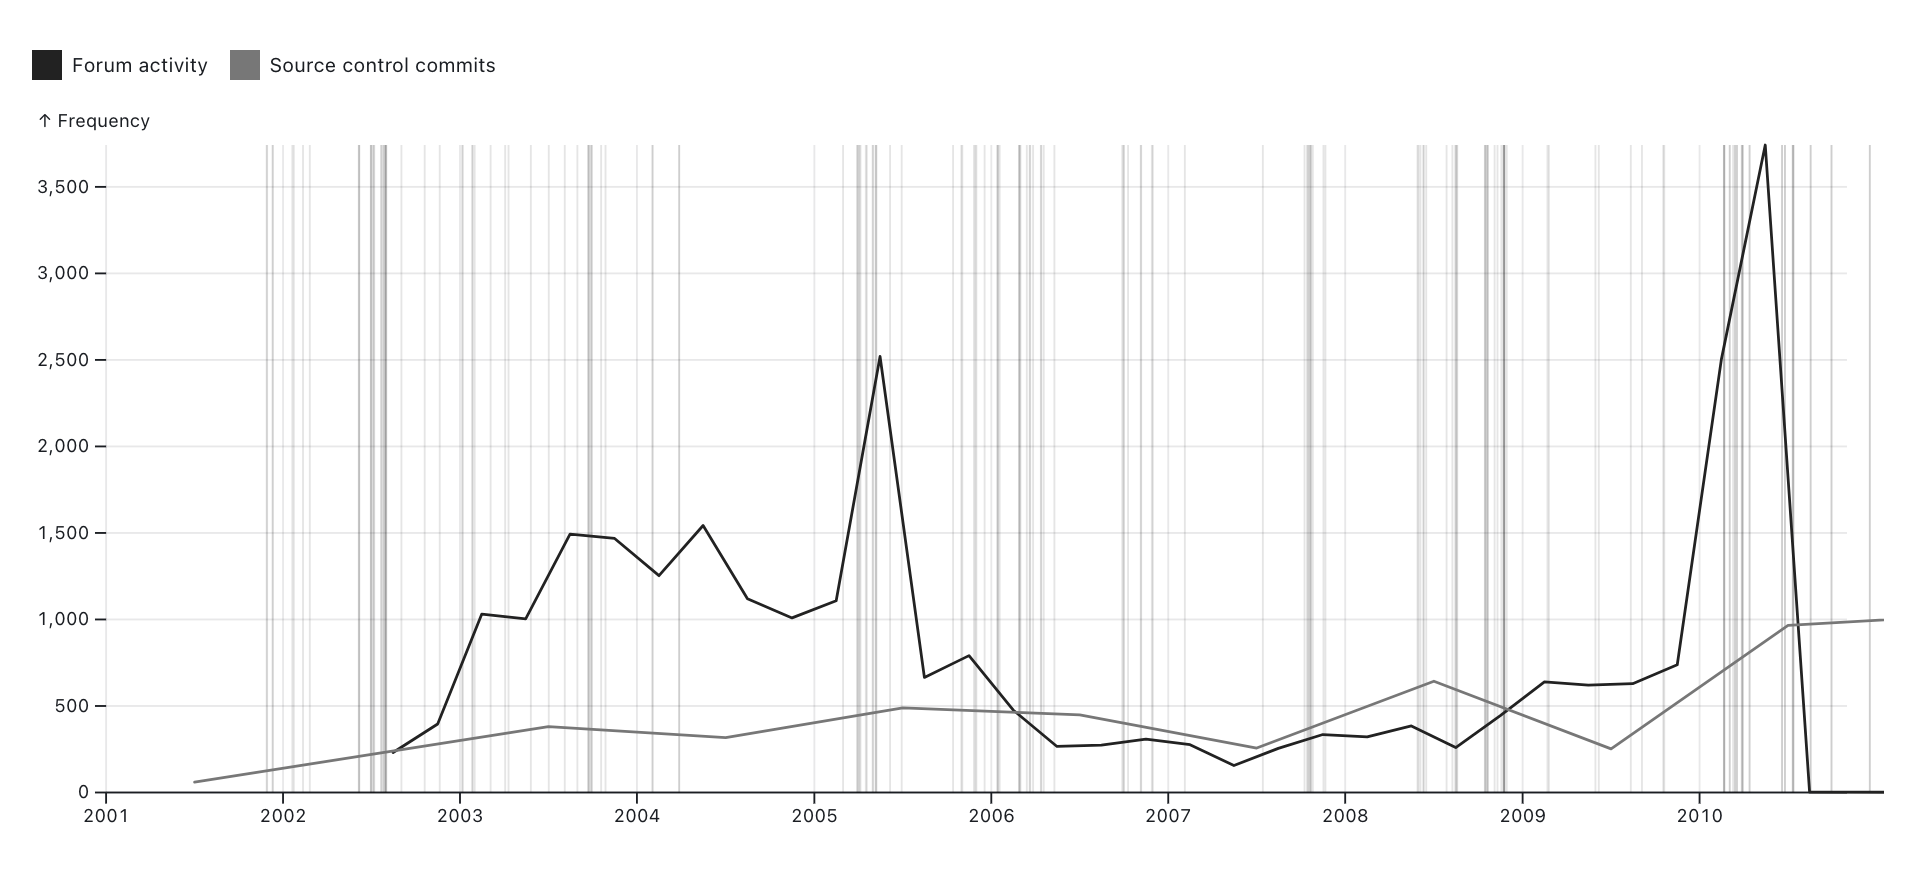
\includegraphics[width=1\textwidth]{images/figure-forum-git-activity.png} 

    \caption{Forum vs git activity vs releases (vertical lines)}
    \label{figure:forum-git-activity}  
  \end{figure}
      \end{block}
      \begin{block}{Furter Research}
        \begin{itemize}
          \item Employ sentiment analysis and topic extraction via large language models on the forum corpus.
          \item Investigate significant peaks in forum and Git activities.
          \item Conduct a survey among the most active contributors to gather qualitative data.
          \item Arrange interviews for in-depth perspectives.
        \end{itemize}
      \end{block}

      \begin{block}{References}
        \printbibliography
      \end{block} 
    \end{column}
    
  \end{columns}
\end{frame}
\end{document}